\documentclass[dvipsnames, svgnames, x11names]{article}

% URLs and hyperlinks ---------------------------------------
\usepackage{hyperref}
\hypersetup{
    colorlinks=true,
    linkcolor=blue,
    filecolor=magenta,      
    urlcolor=blue,
}
\usepackage{xurl}
%----------------------------------------------------

\usepackage{listings}
\usepackage{xcolor}
\usepackage{color}
\definecolor{dkgreen}{rgb}{0,0.6,0}
\definecolor{gray}{rgb}{0.5,0.5,0.5}
\definecolor{mauve}{rgb}{0.58,0,0.82}
\definecolor{jupyterred}{HTML}{BA2121}
\definecolor{jupyterblue}{HTML}{0000FF}
\definecolor{deepred}{rgb}{0.6,0,0}
\definecolor{builtin}{HTML}{000080}

\lstset{frame=tb,
    language=python,
    aboveskip=3mm,
    belowskip=3mm,
    showstringspaces=false,
    columns=flexible,
    basicstyle=\ttfamily,
    numbers=left,
    numberstyle=\small\color{gray},
    keywordstyle=\bfseries\color{Green4},
    commentstyle=\itshape\color{gray},
    stringstyle=\color{jupyterred},
    breaklines=true,
    breakatwhitespace=true,
    tabsize=4,
    identifierstyle=\color{black},
    morekeywords={with},
    emph=[1]{TokenError},
    emphstyle=[1]\color{jupyterblue},
    emph=[2]{__repr__},
    emphstyle=[2]\color{mauve},
    morekeywords={yield},
    classoffset=1,% starting a new class
    morekeywords={IndexError},
    keywordstyle=\bfseries\color{builtin},
}

\usepackage{multicol}
\usepackage{subfigure}
\usepackage{paralist}
\usepackage{amsmath, amssymb, empheq}
\usepackage{enumitem}
\usepackage{adjustbox}
\usepackage{euler}
\usepackage{graphicx}
\usepackage{float}

\usepackage{xepersian}
\settextfont{Yas}
\newcommand{\modts}{\overset{26}{\equiv}}

\title{تکلیف دوم}
\author{مهدی حق‌وردی}
\date{\today}

\begin{document}
\maketitle
\tableofcontents

\section{}
\textbf{{\large با توجه به سیستم رمزنگاری \lr{DES} به سوالات زیر پاسخ دهید.}}

\begin{enumerate}[label=\alph*)]
\item 
\textbf{تعداد کل عملیات‌های 
\lr{\texttt{xor}}
را بدست آورید.}

از آنجایی که 
\lr{DES}
یک ساختار فیستلی ۱۶ دوری است، در بیرون از تابع 
\lr{F},
۱۶ تا 
\lr{\texttt{xor}} 
قرار دارد. و چون درون تابع
\lr{F}
پس از عملیات 
\lr{extend}
یک بار با کلید 
\lr{\texttt{xor}}
انجام می‌گیرد پس اینجا هم ۱۶ تا عملیات 
\lr{\texttt{xor}}
داریم و در مجموع ۳۲ عملیات 
\lr{\texttt{xor}}.

\item 
\textbf{هدف از 
\lr{s-box}ها
را بنویسید.}

نوشتن رابطه‌ی جبری برای بیت‌‌های خروجی بر حسب بیت‌های ورودی و کلید \textbf{به دلیل وجود \lr{s-box}} بسیار دشوار است.

\item 
\textbf{پیچیدگی حمله‌ی جست‌وجوی جامع به این سیستم از چه مرتبه‌ای می‌باشد؟}

کلید 
\lr{DES},
۶۴ بیتی است که ۸ بیت آن بیت‌های 
\lr{parity}
هستند پس کلید مخفی آن تنها ۵۶ بیت طول دارد $\leftarrow$ جستجوی کامل در 
\lr{DES} 
از مرتبه‌ی 
$2^{56}$
است.

\item 
\textbf{دلیل استفاده از 
\lr{expansion s-box}
در 
\lr{DES Function}
چیست؟}

کلید ۵۶ بیتی 
\lr{DES}
توسط 
\lr{Key Scheduler}
به ۱۶ کلید ۴۸ بیتی تبدیل می‌شود و از آنجایی که طول بلاک 
\lr{DES}
۶۴ بیت است و در ساختار فیستل تنها ۳۲ بیت آن به داخل تابع 
\lr{F}
می‌رود باید ۳۲ بیت ورودی را به ۴۸ بیت گسترش بدهیم تا بتوانیم آن را با کلید 
\lr{\texttt{xor}}
کنیم.

\item 
\textbf{اگر خروجی سیستم رمزنگاری به یک سیستم رمزنگاری دیگر داده شود، چه تغییری در
امنیت آن حاصل می‌شود؟ \lr{(double des)} اگر این کار سه بار تکرار شود
چطور؟ 
\lr{(triple des)}}

\begin{itemize}
\item \lr{double des}

در این حالت برای شکستن می‌توان از حمله‌ی تطابق در میانه استفاده کرد که مرتبه‌ی آن از 
$2^{112}$
به
$2^{57}$ 
تقلیل می‌یابد.

\item \lr{triple des}

در این حالت هم (با استفاده از حمله‌ی تطابق در میانه) مرتبه بجای 
$2^{168}$
می‌شود:
$2^{112}$ که البته در عمل قابل انجام نیست. در سال ۲۰۱۷ 
\lr{NIST}
منسوخ شدن
\lr{3DES}
را اعلام کرد.

\end{itemize}
\item 
ویژگی مکمل بودن این سیستم را ثابت کنید و توضیح دهید در آن صورت حمله به
این سیستم از چه مرتبه‌ایست و چرا؟

خاصیت مکمل بودن 
\lr{DES}:
\begin{latin}
\begin{equation}
\text{DES}_\text{K}(\text{M}) = \text{C}
\Rightarrow
\text{DES}_{\overline{\text{K}}}(\overline{\text{M}}) = \overline{\text{C}}
\end{equation}
\end{latin}

(برای اثبات فقط یک دور را در نظر میگیریم) با توجه به ساختار فیستلی 
\lr{DES}
ورودی ابتدا به دو قسمت تقسیم میکند و سپس نیمه‌ی راست را (درون تابع \lr{F}) با کلید 
\lr{\texttt{xor}}
می‌کند و سپس خروجی را با قسمت سمت چپ 
\lr{\texttt{xor}}
می‌کند.
\begin{center}
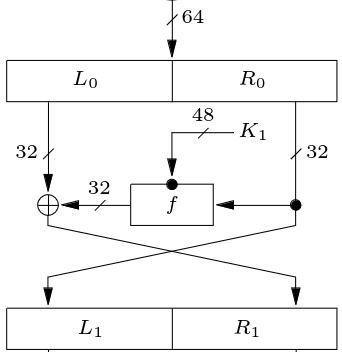
\includegraphics[width=0.4\textwidth, height=0.35\textheight]{des-feistel}
\end{center}
که یعنی:
\begin{equation}
\begin{cases}
P = L_0.R_0\\
L_1 = R_0 \\
B = f(R_0 \oplus K_1) \\
R_1 = L_0 \oplus B
\end{cases}
\Rightarrow C = L_1.R_1
\end{equation}

حال اگر 
\lr{$P$}
و 
\lr{$K$}
را 
\lr{\texttt{not}}
کنیم:
\begin{equation}
\begin{cases}
\overline{P} = \overline{L_0.R_0}\\
L_1 = \overline{R_0} \\
B = f(\overline{R_0} \oplus \overline{K_1}) \\
R_1 = \overline{L_0} \oplus B
\end{cases}
\Rightarrow \overline{C} = \overline{L_1.R_1}
\end{equation}

پس در نتیجه:
\begin{equation}
E_k(P) = C \iff E_{\overline{k}}(\overline{P}) = \overline{C}
\end{equation}
\end{enumerate}

\section{}
{\large \textbf{با استفاده از یک کلید رمز واحد، هر یک ازتبدیلات زیر را بر متن آشکار که تنها در بیت اول با هم تفاوت دارند، اعمال کنید. تعداد بیت‌های تغییر یافته پس از هرتبدیل را پیدا کنید. هرتبدیل را بطور مستقل اعمال کنید. در مورد اثر بهمنی پس از هرتبدیل بطور مستقل و سپس اثر بهمنی پس از اعمال یک راند توضیح دهید.}}

برای نوشتن این سوال هر عملیات 
\lr{AES}
را در پایتون پیاده سازی کردم که 
\lr{source code}
آن در پوشه‌ی 
\lr{\texttt{AES}}
همراه تکلیف ارسال شده است.

پاسخ هر بخش در تصویری که جلویش نوشته شده‌ است نوشته شده است.

\subsection{توضیح تصاویر}
\begin{multicols}{2}
اول از همه نام عملیات در بالای تصویر نوشته شده است،

سپس متن آشکار و متن تغییر یافته و کاراکتر‌هایی که تغییر یافته‌اند نشان داده شده‌اند،

دوباره همین کار روی متن آشکاری که بیت اول آن فرق کرده است تکرار شده است،

سپس تفاوت‌های بین دو متن تغییر یافته نوشته شده،

و در آخر در جدولی تعداد بیت‌های تغییر یافته و درصد تغییر یافتن متن رمز شده‌ی دوم نوشته شده است.

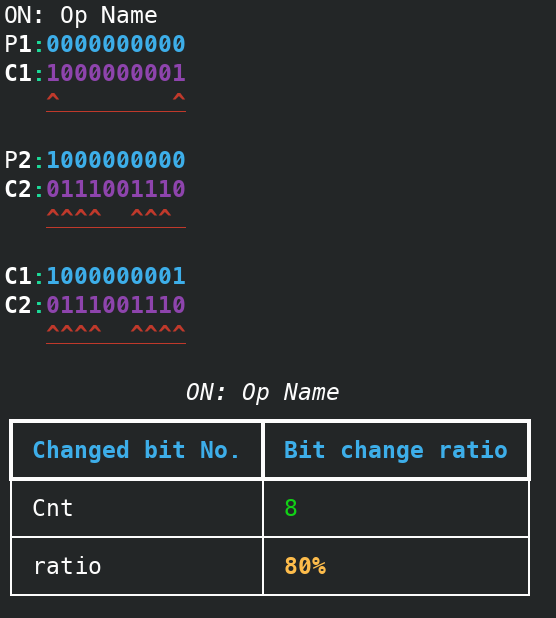
\includegraphics[width=0.45\textwidth, height=0.35\textheight]{exam}
\end{multicols}

\subsection{پاسخ‌ها}
\begin{enumerate}[label=\alph*)]
\item \lr{SB: Sub Byte}
تصویر
\ref{fig:sb}

\item \lr{SR: Shift Row}
تصویر
\ref{fig:sr}

\item \lr{MC: Mix Columns}
تصویر
\ref{fig:mc}

\item \lr{ARK: Add Round Key}
تصویر
\ref{fig:ark}

\item \lr{FR: Full Round}
تصویر
\ref{fig:fr}
\end{enumerate}

همانطور که مشاهده شد، اثر بهمنی در عملیات‌های مختلف درصد کمی داشته و در یک دور (آن هم در این مورد خاص که اولین بیت تغییر کرده است) به 18\% رسید.

اگر ما با کلیدی ۱۲۸ بیتی و عملیات کامل رمزنگار
\lr{AES}
که شامل ۱۶ دور است، (طبق مستندات) اثر بهمنی به نزدیک حداکثر آن، یعنی 50\% می‌رسد.


\begin{figure}[b]
\begin{center}
\subfigure
[\lr{SB: Sub Byte}]
{\label{fig:sb}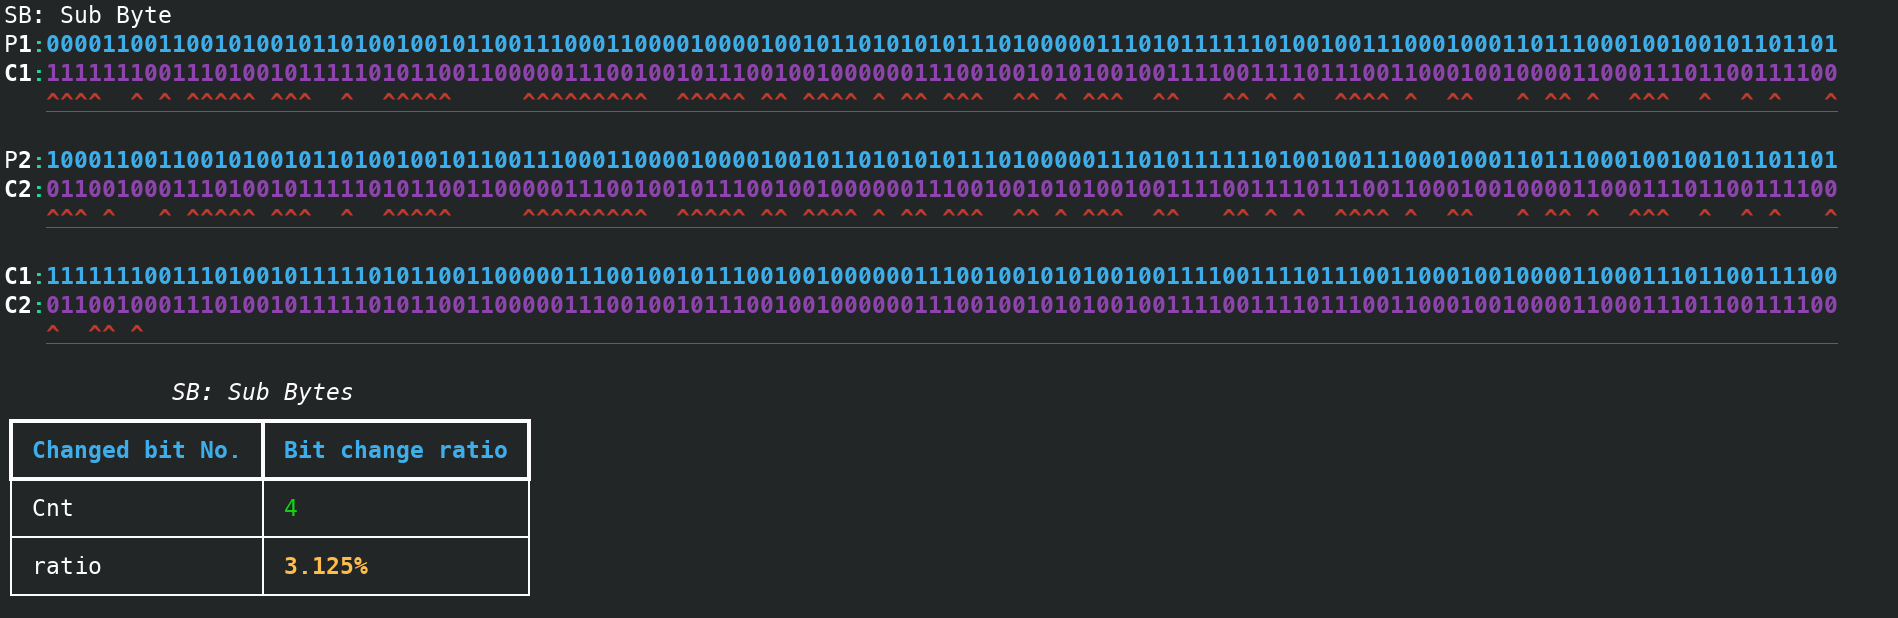
\includegraphics[width=0.8\textheight, height=0.49\textwidth, angle=90]{sb}
}
\subfigure
[\lr{SR: Shift Row}]
{\label{fig:sr}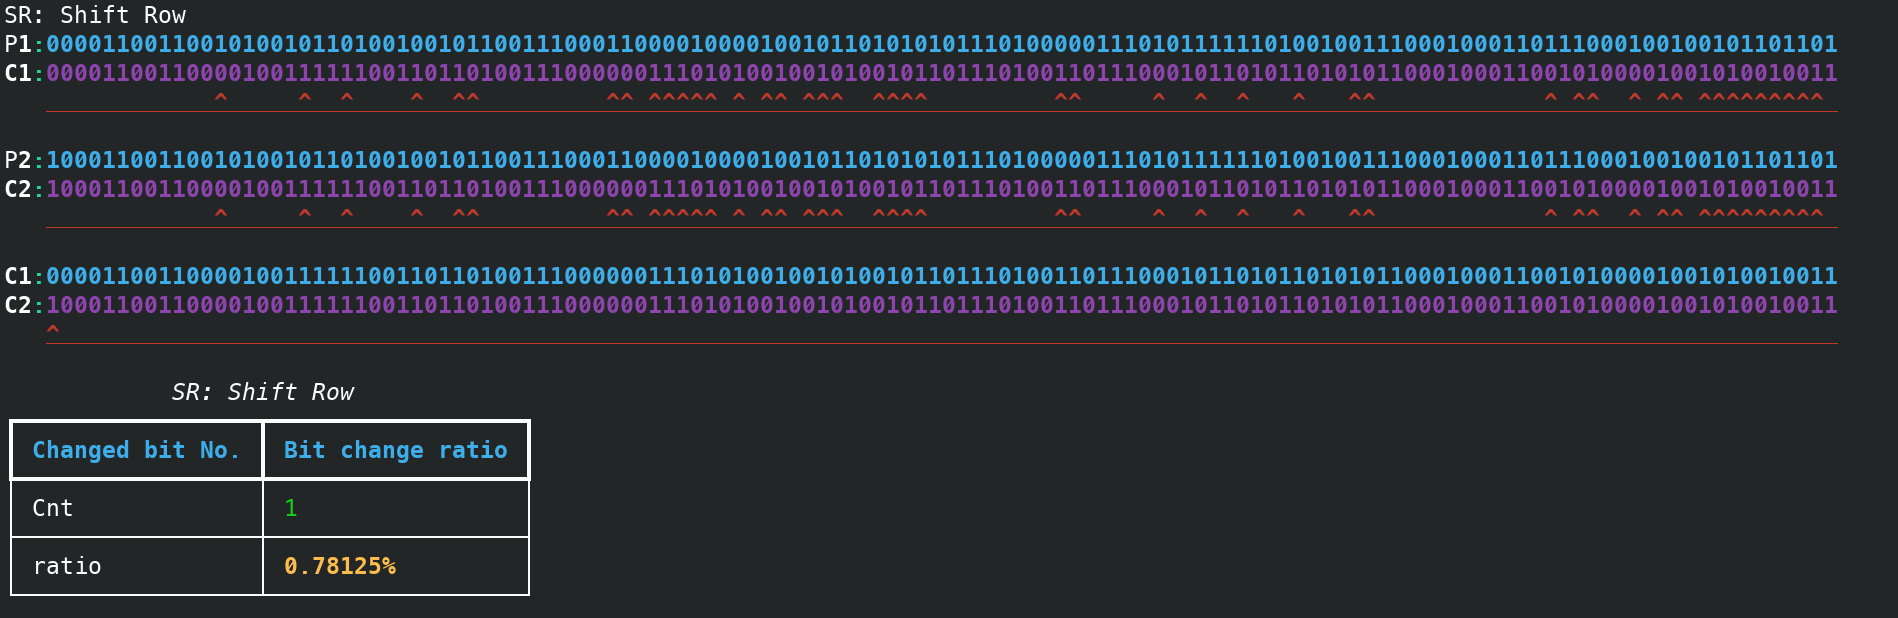
\includegraphics[width=0.8\textheight, height=0.49\textwidth, angle=90]{sr}}
\end{center}
\end{figure}

\begin{figure}[b]
\begin{center}
\subfigure
[\lr{MC: Mix Column}]
{\label{fig:mc}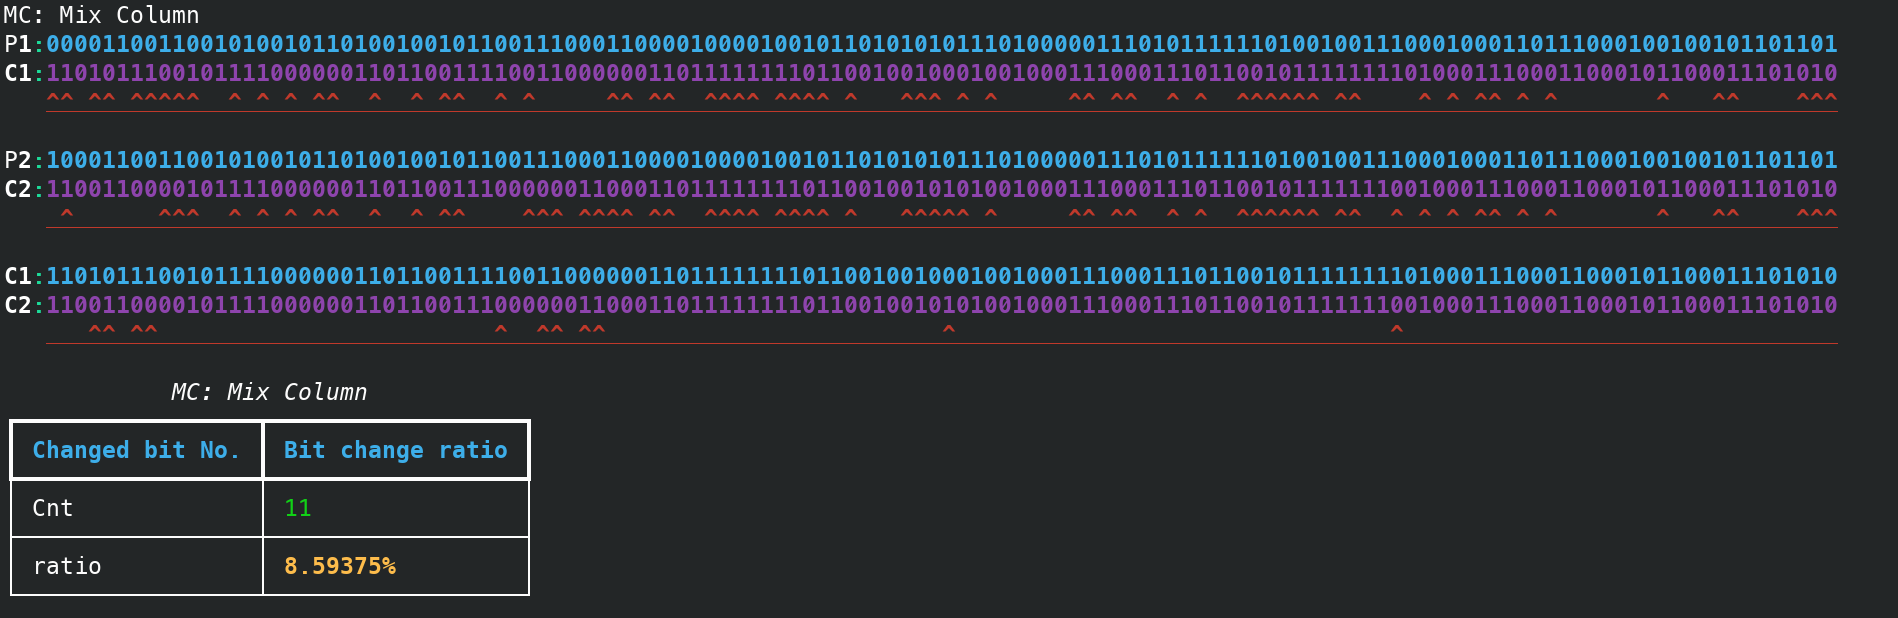
\includegraphics[width=0.8\textheight, height=0.49\textwidth, angle=90]{mc}}
\subfigure
[\lr{ARK: Add Round Key}]
{\label{fig:ark}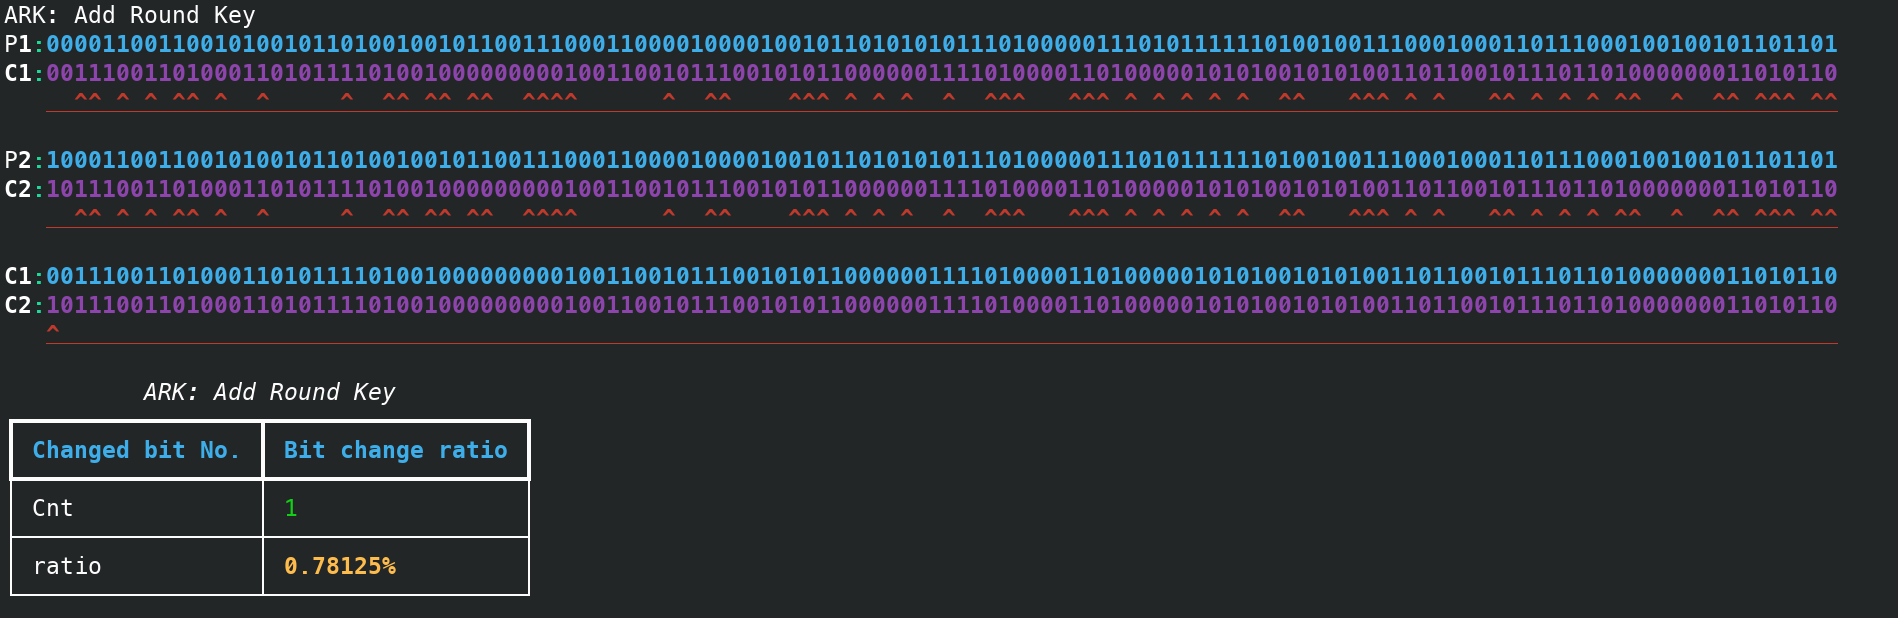
\includegraphics[width=0.8\textheight, height=0.49\textwidth, angle=90]{ark}}
\end{center}
\end{figure}

\begin{figure}[b]
\begin{center}
\subfigure
[\lr{FR: Full Round}]
{\label{fig:fr}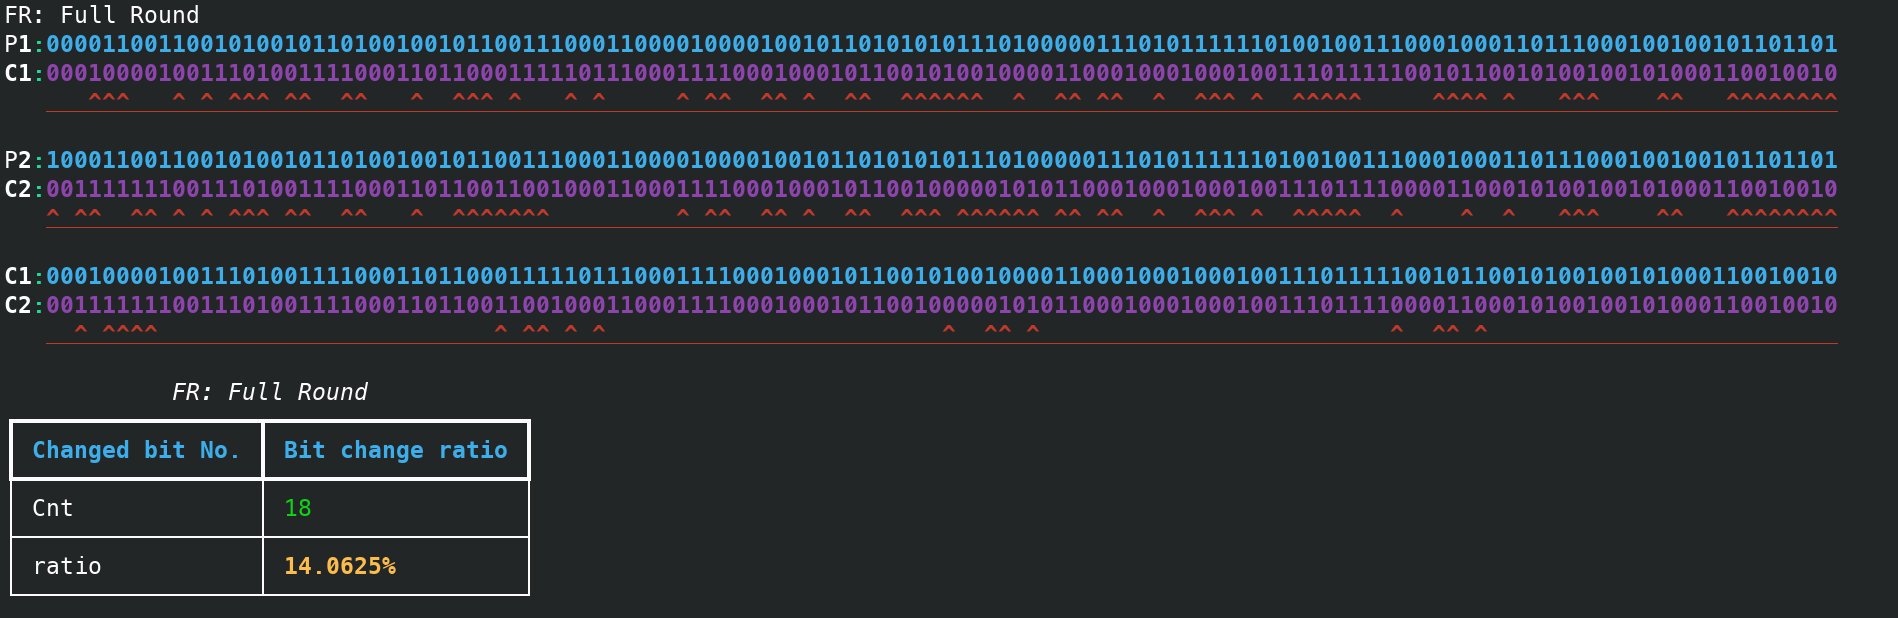
\includegraphics[width=0.8\textheight, height=0.49\textwidth, angle=90]{fr}}
\end{center}
\caption{جزئیات یک دور از \lr{AES}}
\end{figure}

\section{}
{\large \textbf{از بین مدهای عملیاتی
\lr{ECB},
\lr{CBC},
\lr{OFB},
\lr{CFB}
و
\lr{CTR}
در کدام یک امکان افزایش سرعت در عمل رمزگذاری با استفاده از
\lr{parallel processing}
یا پردازش موازی وجود دارد؟}}

مدهای:
\begin{inparaitem}
\item \lr{ECB}
\item \lr{CTR}
\end{inparaitem}

\section{پیوست‌ها}
\begin{latin}
\begin{lstlisting}
"""This module implements 4 operations present in AES
- SB: Sub Bytes
- SR: Shift Rows
- MC: Mix Columns
- ARK: Add Round Key
- FR: Full Round (on of the 16 rounds)
"""

from functools import wraps
from inspect import getfullargspec
from itertools import islice
from typing import TypeAlias

import galois

__all__ = ['sub_bytes', 'isub_bytes', 'shift_row', 'mix_column', 'add_round_key', 'full_round']

BitMat: TypeAlias = list[list[int]]
GF128 = galois.GF(2, 8, irreducible_poly='x^8 + x^4 + x^3 + x + 1')


def batched(iterable, n):
    # batched('ABCDEFG', 3) -> ABC DEF G
    it = iter(iterable)
    while batch := tuple(islice(it, n)):
        yield batch


def stream_to_matrix(stream: str) -> BitMat:
    """Make the stream a matrix converted as an integers

    Arguments:
        stream: b0b1b2...b15

    Return:
        [[b0, b4, b8, b12],
         [b1, b5, b9, b13],
         [b2, b6, b10, b14],
         [b3, b7, b11, b15]]
    """
    ranges = []
    s = 0
    for i in range(0, 128 // 8):
        e = s + 8
        ranges.append((s, e))
        s = e

    mat = [[], [], [], []]
    for r in batched(ranges, 4):
        for idx, ra in enumerate(r):
            s, e = ra
            _stream = int(stream[s:e], 2)
            mat[idx].append(_stream)
    return mat


def matrix_to_stream(matrix: BitMat) -> str:
    """Make the matrix a stream

    Arguments:
        matrix: [[b0, b4, b8, b12],
                 [b1, b5, b9, b13],
                 [b2, b6, b10, b14],
                 [b3, b7, b11, b15]]

    Return:
        'b0b1b2b3...b15'
    """
    stream = ''
    for col in range(4):
        _stream = ''
        for row in matrix:
            _stream += f'{bin(row[col])[2:]:0>8}'
        stream += _stream
    return stream


def type_and_len_check(func):
    @wraps(func)
    def wrapper(*args):
        argnames = getfullargspec(func).args
        for arg, name in zip(args, argnames):
            if not isinstance(arg, str):
                raise TypeError(f'{name!r} should be `str`')

        for arg, name in zip(args, argnames):
            if not len(arg) == 128:
                raise ValueError(f'{name!r} should 128 bits')

        return func(*args)

    return wrapper


############ SB: Sub Bytes ############  # noqa: E266
sb_mat = GF128(
    [[1, 0, 0, 0, 1, 1, 1, 1],
     [1, 1, 0, 0, 0, 1, 1, 1],
     [1, 1, 1, 0, 0, 0, 1, 1],
     [1, 1, 1, 1, 0, 0, 0, 1],
     [1, 1, 1, 1, 1, 0, 0, 0],
     [0, 1, 1, 1, 1, 1, 0, 0],
     [0, 0, 1, 1, 1, 1, 1, 0],
     [0, 0, 0, 1, 1, 1, 1, 1]],
)

isb_mat = GF128(
    [[0, 0, 1, 0, 0, 1, 0, 1],
     [1, 0, 0, 1, 0, 0, 1, 0],
     [0, 1, 0, 0, 1, 0, 0, 1],
     [1, 0, 1, 0, 0, 1, 0, 0],
     [0, 1, 0, 1, 0, 0, 1, 0],
     [0, 0, 1, 0, 1, 0, 0, 1],
     [1, 0, 0, 1, 0, 1, 0, 0],
     [0, 1, 0, 0, 1, 0, 1, 0]],
)

b = GF128([[1], [1], [0], [0], [0], [1], [1], [0]])
ib = GF128([[1], [0], [1], [0], [0], [0], [0], [0]])


def _sub_byte(byte: int) -> int:
    """SubByte the integer according to s(x) = ax^(-1)+b"""
    number = GF128(byte)
    rev = GF128(number) ** -1 if byte != 0 else 0
    mat = GF128([[char] for char in reversed(f'{bin(rev)[2:]:0>8}')])
    _result = (sb_mat @ mat) + b
    num = ''
    for bit in reversed(_result):
        num += str(bit[0])
    return int(num, 2)


def _isub_byte(byte: int) -> int:
    number = GF128(byte)
    mat = GF128([[char] for char in reversed(f'{bin(number)[2:]:0>8}')])
    _result = (isb_mat @ mat) + ib
    num = ''
    for bit in reversed(_result):
        num += str(bit[0])
    rev = int(num, 2)
    res = GF128(rev) ** -1 if byte != 0 else 0
    return res


def _sub_bytes(input_stream: BitMat) -> BitMat:
    _r = [
        [0, 0, 0, 0],
        [0, 0, 0, 0],
        [0, 0, 0, 0],
        [0, 0, 0, 0]
    ]

    for col in range(4):
        for row in range(4):
            sb = _sub_byte(input_stream[row][col])
            _r[row][col] = sb
    return _r


def _isub_bytes(input_stream: BitMat) -> BitMat:
    _r = [
        [0, 0, 0, 0],
        [0, 0, 0, 0],
        [0, 0, 0, 0],
        [0, 0, 0, 0]
    ]

    for col in range(4):
        for row in range(4):
            sb = _isub_byte(input_stream[row][col])
            _r[row][col] = sb
    return _r


@type_and_len_check
def sub_bytes(stream: str) -> str:
    """Sub byte the stream

    Arguments:
        stream: b1b2b3...b15

    Return: s1s2s3...s15
    """
    _is = stream_to_matrix(stream)
    return matrix_to_stream(_sub_bytes(_is))


@type_and_len_check
def isub_bytes(stream: str) -> str:
    """Inverse sub byte the stream

    Arguments:
        stream: s1s2s3...s15

    Return: b1b2b3...b15
    """
    _is = stream_to_matrix(stream)
    return matrix_to_stream(_isub_bytes(_is))


############ SR: Shift Rows ############  # noqa: E266
def _rotate_left(row: list, rotate: int):
    for _ in range(rotate):
        got = row.pop(0)
        row.append(got)


def _shift_rows(input_stream: BitMat) -> BitMat:
    _input_stream = input_stream.copy()
    for idx, row in enumerate(_input_stream):
        _rotate_left(row, idx)

    return _input_stream


@type_and_len_check
def shift_row(stream: str) -> str:
    """ShiftRow the stream

    Arguments:
        stream: b1b2b3...b15

    Returns:
        stream of:
            [[b0, b4, b8, b12],
             [b5, b9, b13, b1],
             [b10, b14, b2, b6],
             [b15, b3, b7, b11]]
    """
    strm = stream_to_matrix(stream)
    return matrix_to_stream(_shift_rows(strm))


############ MC: Mix Columns ############  # noqa: E266
mc_mat = GF128(
    [[0x02, 0x03, 0x01, 0x01],
     [0x01, 0x02, 0x03, 0x01],
     [0x01, 0x01, 0x02, 0x03],
     [0x03, 0x01, 0x01, 0x02]]
)


def _mix_column(input_stream: BitMat) -> BitMat:
    _r = []
    got = GF128(input_stream)
    _result = got @ mc_mat
    for row in _result:
        _r.append([num for num in row])
    return _r


@type_and_len_check
def mix_column(stream: str) -> str:
    """MixColumn the stream

    Arguments:
        stream: b1b2b3...b15

    Return:
        apply a matrix multiplication and return the stream
        c1c2c3...c15
    """
    _is = stream_to_matrix(stream)
    return matrix_to_stream(_mix_column(_is))


############ ARK: Add Round Key ############  # noqa: E266
@type_and_len_check
def add_round_key(stream: str, key: str) -> str:
    return f'{bin(int(key, 2) ^ int(stream, 2))[2:]:0>128}'


############ FR: Full Round ############  # noqa: E266
def _full_round(input_stream: BitMat, key: str) -> str:
    _sb = _sub_bytes(input_stream)
    _sr = _shift_rows(_sb)
    _mc = _mix_column(_sr)
    _ark = add_round_key(matrix_to_stream(_mc), key)
    return _ark


@type_and_len_check
def full_round(stream: str, key: str) -> str:
    return _full_round(stream_to_matrix(stream), key)
\end{lstlisting}
\end{latin}
\end{document}